% !TEX root = ../thesis_main.tex
%
%
%
%%%% --- * --- %%%%	
\clearpage
\chapter{Atomic Physics Overview}
\label{atomicphysics_chapter}

\note[color=jb]{First, I'm pretty sure you should combine Chs. 3 and 4.
Ch 4 has good solid general description and details in situ about optical
pumping and about the photoionization probe that are,
unfortunately, wrong in Ch. 3.
You could call the first half of such a chapter
"General considerations of Atomic techniques used"
and the 2nd half "Experimental Implementation of Atomic Techniques used"}
\note[color=todoblue]{wtf could I possibly have gotten wrong in my Ch.3 description?  It's so vague!}

\section{Magneto-Optical Traps}
\note[color=org]{I need to organize the sections/subsections in this chapter better...}
Since its initial description by Raab et. al. in 1987~\cite{raabprentiss}, the magneto-optical trap (MOT) has become a widely used technique in many atomic physics laboratories.  The MOT produces confined samples of cold, electrically neutral and isotopically pure atoms confined within a small spatial region.  It is these properties that make the MOT a valuable tool not only in atomic physics, but for precision measurements in nuclear physics as well, and the TRINAT lab \aside[color=org]{Have I defined TRINAT yet?} has adopted the technique wholeheartedly.

The technique is used predominantly with alkalis due to their simple orbital electron structure,% so is appropriate for use with $^{37}\textrm{K}$.  
and once set up it is quite robust.  The MOT's trapping force is specific to the isotope for which the trap has been tuned. This feature makes it ideal for use in precision radioactive decay experiments, since the daughters are unaffected by the trapping forces keeping the parent confined.
\note[color=org]{Possibly most of the above paragraph is also written/paraphrased elsewhere.  Like in Ch-4, unless I removed it...}
%\note{... used predominantly with alkalis due to their simple orbital electron structure.}

A typical MOT can be created from relatively simple components:  a quadrupole-shaped magnetic field, typically generated by two current-carrying coils of wire, and a circularly polarized laser tuned to match one or more atomic transitions in the isotope of interest.  Because a MOT is easily disrupted by interactions with untrapped atoms, the trap must be created within a vaccuum system.  Finally, a source of atoms to be trapped is required.  [See Fig.~\ref{fig:mot}.]

%There are two primary components necessary for any MOT:  a laser, and a magnetic field.  
The laser, which must be circularly polarized in the appropriate directions and tuned slightly to the red of an atomic resonance, is split into three perpendicular retroreflected beams, doppler cooling the atoms and (with the appropriate magnetic field) confining them in all three dimensions (see Figure~\ref{fig:mot}).  
%The TRINAT science chamber includes 6 `viewports' specifically designed to be used for the trapping laser.


\note{``In order to understand the mechanism by which a MOT is able to confine atoms, we must first introduce the Zeeman effect (Section 2.1) and a description of an optical molasses (Section 2.2). A functional MOT combines the forces resulting from these two mechanisms to trap and cool atoms.''}

%The TRINAT lab has adopted this technique from atomic physics to perform nuclear physics experiments.  
%Such samples may subsequently be used in a variety of physical measurements.
%\note{``Since the magneto-optical trap (MOT) was first described in 1987 by Raab et. al.~\cite{raabprentiss}, it has become a standard technique for confining cold samples of neutral atoms.  These cold trapped atoms may subsequently be used in the measurement of a variety of physical quantities."}


\subsection{Zeeman Splitting}
In the presence of an external magnetic field $\vec{B}$, the Hamiltonian associated with an atom's orbital electrons will acquire an additional ``Zeeman Shift'' term, given by~\cite{corney}
\bea
\label{zeeman_hamiltonian}
H_{\mathrm{\,Zeeman}} &=& - \vec{\mu}\cdot \vec{B},
\eea
where $\vec{\mu}$ is the magnetic moment associated with the orbital under consideration.  In the limit where the magnetic field is too weak to significantly disrupt the coupling between the electron's spin- and orbital angular momenta, $\vec{\mu}$ may be treated as being fixed with respect to changes in the magnetic field.  It is this weak field regime which will be primarily of interest to us in work with magneto-optical traps.


With $\vec{\mu}$ fixed, it is clear that the magnitude of the energy shift must scale linearly with the strength of the magnetic field.  In considering the perturbation to the energy of a particular \emph{transition}, the perturbations to the initial and final states must of course be subtracted:
\bea
\Delta E_{\mathrm{\,transition}} &=& - \left( \vec{\mu}_f - \vec{\mu}_i \right) \cdot \vec{B}.
\eea 



%an atom's orbital energy levels take on a perturbation.  The perturbation to the Hamiltonian is given by
%
%the energy levels associated with an atom's electron orbitals are perturbed.  

%\note{Needs work.}
%\note{Needs an equation.}
\note{Needs a level diagram.  Maybe.}

%The Zeeman shift is what happens when you stick an atom in a magnetic field.  An atom's energy levels, which would have been degenerate before applying a field, split according the angular momentum.  At low fields (which is what is of interest to us here), the energy perturbation scales linearly with the strength of the magnetic field.  

\note{
When this is combined with a circularly polarized laser beam, the effect is to move the atomic resonance closer to- or farther from- the frequency of the laser.  The circular polarization, combined with some selection rules, means a circularly polarized laser will only couple to one particular transition, w.r.t. angular momentum.  ie, for a $\sigma_+$ polarized laser, the atom's overall angular momentum projection (along some axis) will be incremented by $+1$.  The Zeeman shift means that in a magnetic field, this transition (M+=1) not be the same as the M-=1 transition.  So, if you have a magnetic field that changes linearly across space, you can make it so that in $+ B_z$ regions, the laser beam with one certain polarization is closer to resonance and therefore more likely to be absorbed -- and similarly, in $- B_z$ regions, a different laser with the opposite polarization will be more likely to be absorbed.  Again, if the B-field is linear in space, you can do it so that as the atoms get further and further from the `centre' region, the effect gets progressively stronger.  So, if you've done this right, you can make it so that the atoms get a stronger ``push'' back towards the center the farther away they've drifted.
\\
They still get the optical molasses cooling effect for free.}


\subsection{Atom-Photon Interactions within a Laser}
\note[color=jb]{JB says:  Chapter 3 (that's this chapter):
Starting in Ch. 3 around p. 10, "Atom-Photon Interactions with a Laser" (that's this section):
\\
You need to do a careful pass through it and omit everything you don't
understand and don't need.
\\
Sorry, there is no longer time to resolve your questions unless you need them.}

\note{This is a stupid subsection title.}
%We consider first the interaction between a single atom and a single photon.  Suppose 

Consider a single two-level atom in its ground state interacting with a single photon with the same energy as that of a the atomic transition between the ground and excited states.  If angular momentum selection rules allow it\aside{Also, if the photon is tuned close enough to atomic resonance, with absorption being more likely the smaller the detuning is...}, the photon will be absorbed and the atom will receive a ``push'' 
from the incident 
%
%proportional to the 
%detuning\aside{Wait.  I don't think I got that right.  Detuning only affects absorption probability, right?  I guess it also has an effect on the size of the push, but that's really not the primary pushing effect going on here.} of the photon from the atomic resonance.  
%
photon's momentum.  
After a time, the atom will spontaneously de-excite by emitting a photon in a random direction.  Conservation of momentum results in the atom receiving a second push from the emitted photon.  

If one considers a cloud of many such atoms within the path of a correctly-tuned (low intensity) laser beam, then provided the atoms are constrained to remain within the beam path, the result of many such interactions is a biased random walk in physical space for each individual atom, and a net velocity change for the cloud as a whole.
% such that the cloud as a whole receives a change in net velocity. 

In contrast to the above description of absorption followed by spontaneous emission, a photon interacting with an atom in the excited state may cause the atom to de-excite by emitting a second photon.  This mechanism is negligible in the case of a sufficiently low intensity laser beam.  However, as the laser intensity increases, so too will the fraction of atoms in the excited state at any given time.  As it is only the excited state atoms that are able undergo stimulated emission, this effect becomes increasingly dominant as the intensity of the incident laser increases.  In the limit of infinite intensity, stimulated emission and absorption are equally likely to occur, and therefore the population is split evenly between the ground and excited states.  

To describe the regime change between atomic interactions with low intensity- and high intensity lasers, we introduce the (on-resonance) saturation intensity, $I_{\mathrm{sat}}$, where 
\bea
I_{\mathrm{sat}} &=& \frac{\hbar \omega_0^3 \gamma}{12\pi c^2}
\eea
is the laser intensity at which the rates of decay by stimulated- and spontaneous emission are equal, $\hbar \omega_0$ is the energy of both the atomic transition %and also an individual photon, 
and $\gamma$ describes the linewidth of the atomic transition and equivalently its rate of spontaneous decay from its excited state.  We may further define the on-resonance saturation parameter $s_0$, for a laser of intensity $I$ as,
\bea
s_0 &:=& \frac{I}{ I_{\mathrm{sat}} }.
\eea

In practice, for the project that is the topic of this thesis, the MOT laser operates at about 1/2 of saturation intensity, while the optical pumping
and photoionization lasers operate at considerably lower than saturation
intensity. However, one can gain
%most lasers operate in the high intensity regime -- the obvious exception being the photoionization laser (see Section whatever)
%\aside[color=org]{Where have I even decided to put the photoionization section, anyway?}  
%However, one can still gain 
a qualitative understanding of many aspects of atom-laser interaction while neglecting saturation concerns.  
\note[color=done]{Fixed description of which lasers are saturated.}
%\aside{Clunky phrasing.} 
%\aside[color=todoblue]{Do I need saturation to make an optical molasses?  I bet I do.}  
\note{Do I need to mention saturation at all?  It's probably not really necessary, and I don't *think* anything else in this section is wrong per se.  But maybe better to just cut it.}

%\note[color=jb]{JB says:  "In practice, for the project that is the topic of this thesis,
%most lasers operate in the high intensity regime –
%the obvious exception being the photoionization laser (see Section whatever)
%However, one can still gain ..."
%\\
%change to ->
%\\
%"In practice, for the project that is the topic of this thesis,
%the MOT laser operates at about 1/2 of saturation intensity,
%while the optical pumping
%and photoionization lasers operate at considerably lower than saturation
%intensity.
%However, one can gain ..."}
%
% % % 

\subsection{Doppler Cooling}
% % % 
We now consider a somewhat more general case in which a cloud of two-level atoms lies along the path of two counter-propagating laser beams, both detuned slightly to the red of resonance.  For simplicity, this cloud will be treated as being constrained in the other two dimensions such that it must within the laser's path.  With two counter-propagating laser beams of equal intensity and detuning,\aside{...and opposite polarization.  Or something.  I have to talk about the selection rules somewhere else.} the ``push'' from interaction with one beam is exactly counteracted by the push from the opposite-propagating beam, and there is no net velocity transfer to the cloud.  

Detuning the laser from resonance will of course decrease absorption upon interacting with an atom at rest -- however the atoms within the cloud are not at rest, but rather are undergoing thermal motion.  As such, within the rest frame of each individual atom, the two laser beams will appear to be Doppler shifted in opposite directions, with the sign dependent on atomic motion.  In particular, atoms moving against a laser's direction of propagation will see that laser beam as being blueshifted.  Since the laser has been red-detuned within the lab frame, the blueshift moves the laser frequency as seen by the atom back toward resonance, and makes its photons more likely to be absorbed.  Similarly, for an atom moving in the same direction as a red-detuned laser beam, this laser will be seen as further red-shifted, and absorption likelihood is decreased.  Because of the difference in absorption, such an atom becomes more likely to receive a push back against its (lab frame) direction of motion, slowing it down, and less likely to recieve a push to increase its lab frame speed.   \aside{Optical molasses equation?  Maybe?}

The overall effect on a one-dimensional cloud of atoms in the path of two counter-propagating red-detuned lasers is that the atoms will be slowed and cooled.  Such a setup is sometimes referred to as a one-dimensional ``optical molasses'' due to the viscous drag force induced on atomic motion.  It is straightforward to extend this model to three dimensions.  Although this setup will decrease atomic velocity, it does not include a confining force, so the atoms are still free to move out of the lasers' path, albeit at a decreased speed.  


%The laser's red detuning with respect to the atomic resonance 

%being used are of a sufficiently high intensity  
%\note{``Such a setup is sometimes referred to as a one-dimensional “optical molasses” due to the viscous drag force induced on atomic motion, which will be discussed in more detail shortly.''}
%\note{``In such a system, an incident photon can excite an atom from the ground state into the excited state, while simultaneously giving the atom a “push” proportional to the laser’s detuning from the atomic resonance.''}

%Consider an atom in one dimension in the midst of two counter-propagating laser beams which are otherwise identical.   ...Ugh.
\note{``...This will slow the atom down, at least up to a limit related to the linewidth of the atomic transition and/or the laser.  There's something to look up.''}
%\note{Needs an equation. (?)}
%\note{Needs work.}
%\note[color=org]{I should really split these things back up into subsections.  Zeeman shift, saturation intensity, optical molasses/doppler cooling.  Then selection rules.}

%First, consider an atom in an optical molasses.  in 1D, that means there are two counter-propogating lasers, both tuned slightly to the red of an atomic transition.  Also, they're polarized s.t. ... something.  The point is, atoms moving against the direction of a red-detuned laser's propagation will see a doppler shifted laser frequency, tuned closer to the atomic transition, which makes a photon more likely to be absorbed.  Similarly, the opposite-propagating laser will appear to be further red-shifted away from resonance.  When a photon is absorbed, we require conservation of (linear) momentum, so the atom gets a ``push'' against the direction it was travelling.  This will slow the atom down, at least up to a limit related to the linewidth of the atomic transition and/or the laser.  There's something to look up.
%
%Anyway, when you have two counter-propagating red-detuned lasers, the net effect will be to slow the atom's motion down a bunch.  It's called an optical molasses, because the photons are sticky or whatever.  By itself, it does not confine atoms, it only slows them down.

%%%% % % % %%%
%\subsection{Angular Momentum and Selection Rules}
%\note[color=jb]{JB:  3.1.4 Angular Momentum and Selection Rules (that's this section!):
%\\
%Sorry, this section is almost entirely wrong, and you don't need it.
%Omit it please.}
%
%\note[color=jb]{JB:  Agreed it's ok to ignore the repumper laser.}
%
%As in any other interaction, when a photon and an atom interact with one another, angular momentum must be conserved.
%%In any interaction, angular momentum must be conserved, and the interactions between atoms and photons are no exception.  
%An individual photon has spin 1, and therefore when we consider an atom-photon interaction where the photon is absorbed, the atom's total angular momentum projection \comment{(I think on any axis???)} must also change by one unit.
%\note{Fuck.  What even *are* the other rules?  Have to change F too?  I think that's true.. Clearly I have to look this up.}
%On a macroscopic level, the polarization of a laser can be used as a stand-in to describe, in a probabilistic way, the spin orientation of the individual photons of which the beam consists.  
%
%\note{I mean.  I probably don't need to go too in-depth here.  But I haven't mentioned it at all yet, and it's a relevant thing.}
%Polarization matters.  You have to conserve angular momentum.  In fact, you have to conserve both total angular momentum *and* its projection on whatever axis.  Photons have spin-1, but because they literally go at the speed of light, they can't do $0 \rightarrow 0$ transitions.  
%
%This is related to why you need repumpers for your MOT, but also, I don't really want to get into that.  But also-also, why even *would* you?  You don't in the description I've already given.  Pretty sure it's because you can sometimes de-excite to a *stupid* set of energy levels.  And then, I don't think they really fall back down or something?  I've largely forgotten how it works.  Ugh.
\note[color=done]{Removed `Angular Momentum and Selection Rules' section.  Because it was super wrong.}

%%% % % % %%%
\section{Optical Pumping}
\label{sec:op}
\note[color=jb]{3.2 (that's this section!):
\\
You cover what is needed for optical pumping well in "4.2 the AC MOT and Poalrization setup"
Just say here indeed
"The optical pumping process is describe in detail in our collaboration's
Ref.~\cite{ben_OP}. The main detail described here is that the
optical pumping is distrubed by any component of magnetic field not along
the quantization axis. (Ours is the vertical axis, defined by the direction
of the optical pumping light, and along which the detectors are placed.)
This required sophistication with an AC MOT described below.
\\ ... \\
Then you can refer to that in section 3.4, where you're trying to now but the phrasing is poor."}

\note{Needs work.}
\note{``Until recently, one limitation of such samples was the necessity for the presence of a relatively large magnetic field, which is expected to partially destroy atomic polarization, limiting the precision of many types of measurements.  Here we discuss the construction of a newer type of MOT, the AC-MOT, which minimizes residual magnetic fields.  The guys in~\cite{harveymurray} came up with the idea of the AC-MOT.  They made it work and did some stuff with it.  Good for them.''}
Need a nice, uniform, constant magnetic field for your polarization to larmor precess around.  Then, however depolarized (from the axis of the magnetic field) you were to start out, you don't like precess in a way that changes the projection you care about.

But also, I should actually describe the optical pumping, too.  And point at Ben's OP paper that we did~\cite{ben_OP}.

\note[color=org]{Somewhere later, I can talk about photoionization?  Or should it be here, in this chapter?  Surely it should at least get a different section though.}

%\missingfigure{I need \emph{at least} one atomic level diagram.  But possibly as many as 3 level diagrams.  Have to show energies for MOT, energies for OP, and energies for photoionization.  }

%\note{Needs a better level diagram.  Or possibly no level diagrams at all.}
%\note{Previous assertion:  I need \emph{at least} one atomic level diagram.  But possibly as many as 3 level diagrams.  Have to show energies for MOT, energies for OP, and energies for photoionization.}
\note{Do I need a MOT level diagram too?}

\begin{figure}[h!!t]
	\centering
	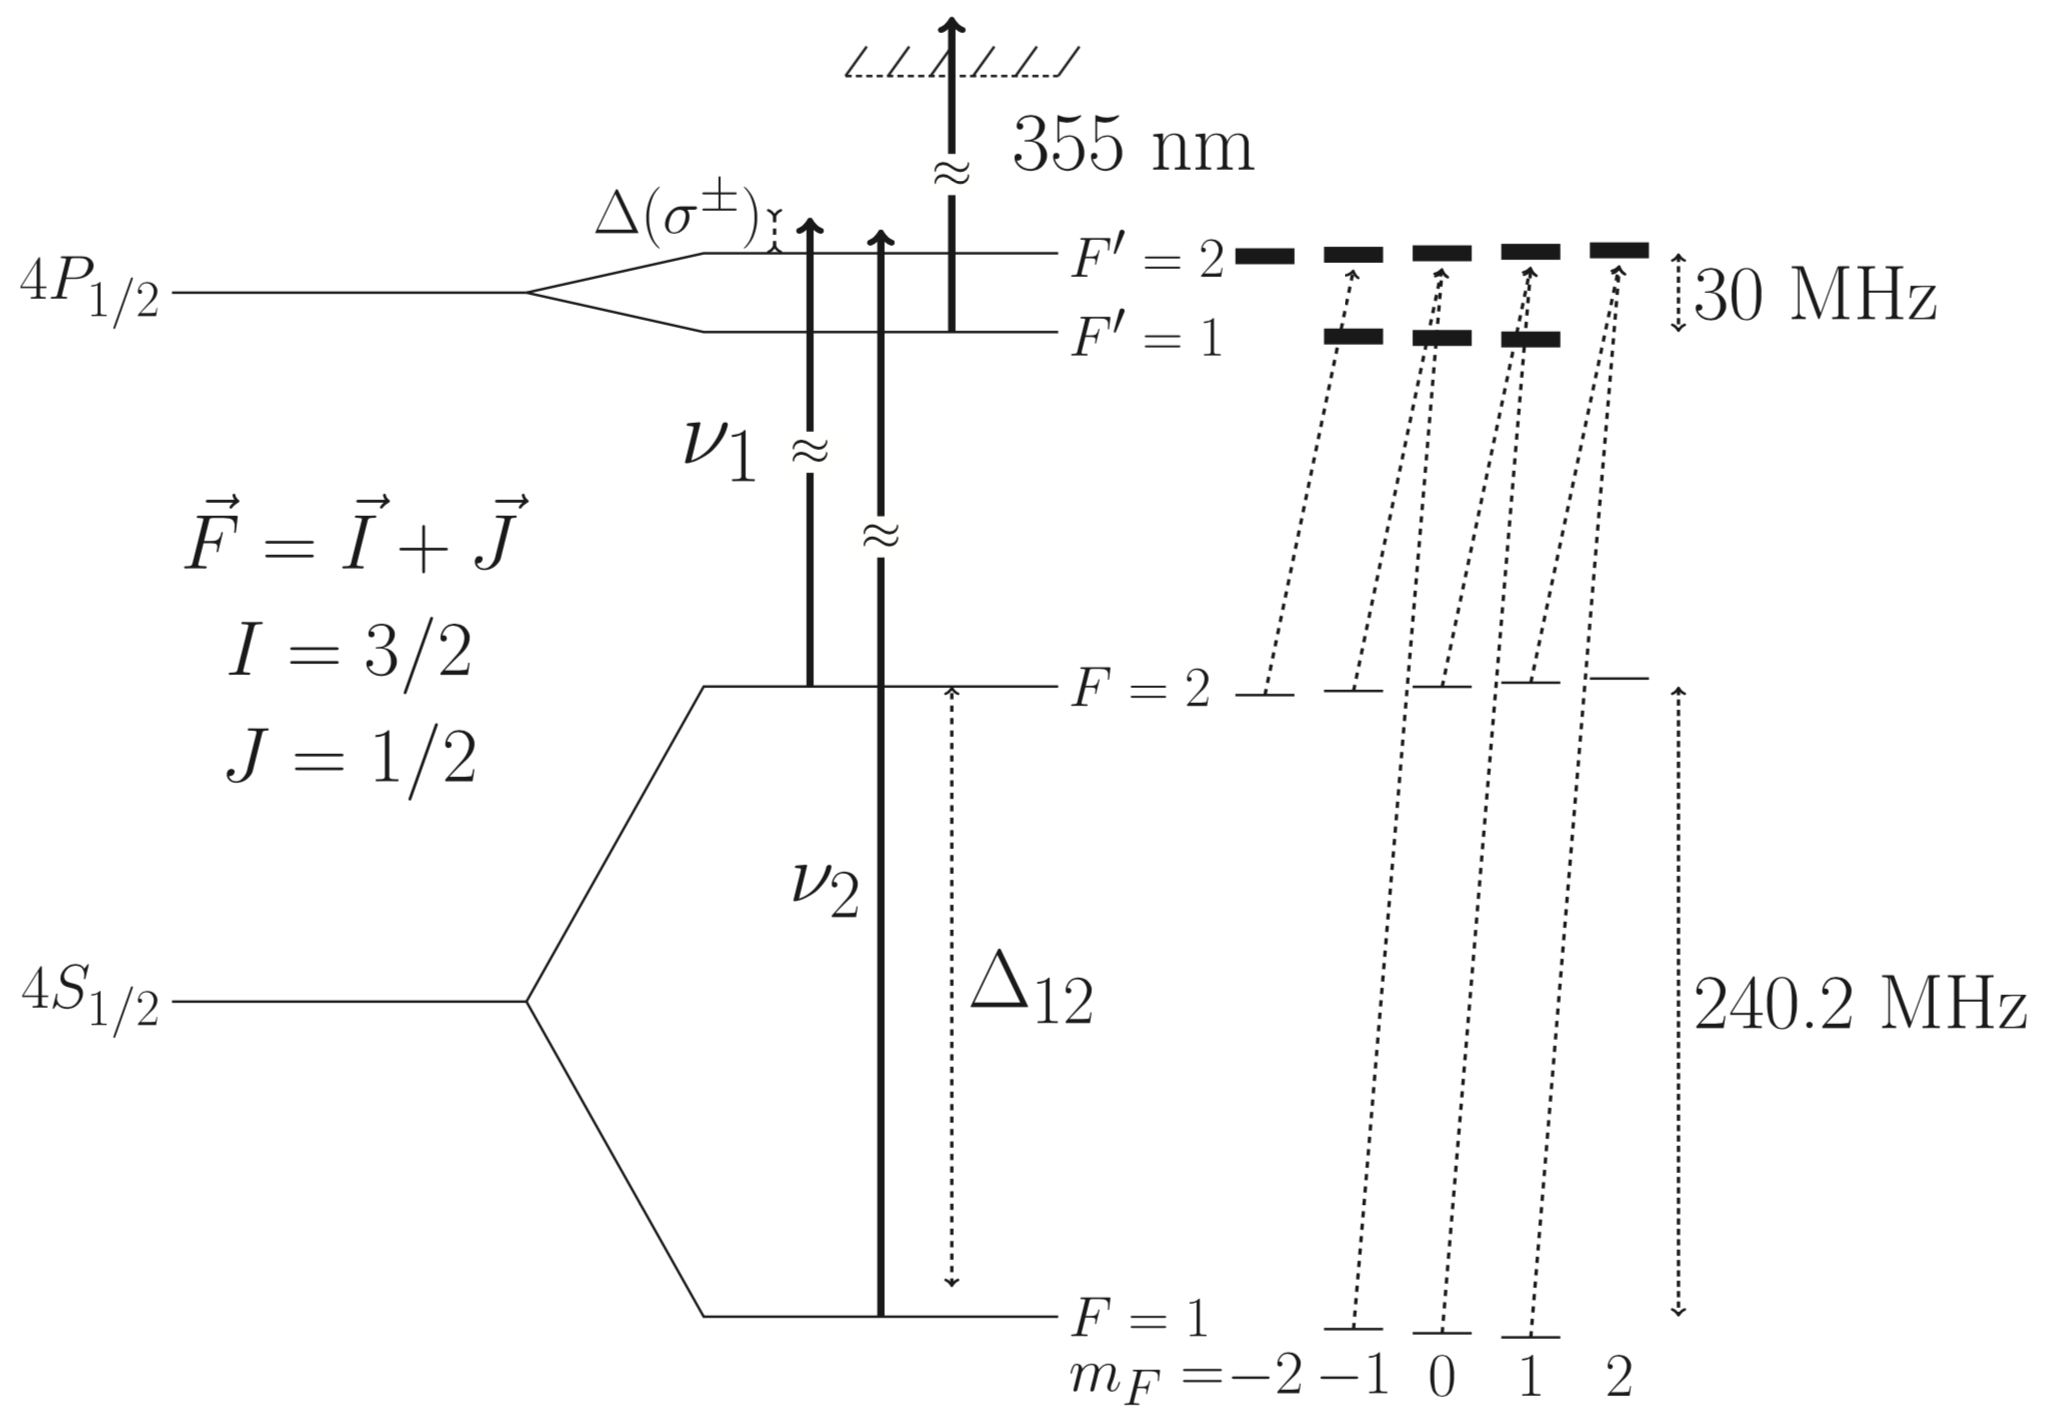
\includegraphics[width=.999\linewidth]
	{Figures/OP_LevelDiagram_bf.png}
	\note{Describe what's going on here!}
	\caption{An atomic level diagram for the optical pumping of $\isotope[37]{K}$, taken from \cite{ben_OP}.  }	
	\label{fig:op_leveldiagram}
\end{figure}

\note[color=purple]{JB says:  ``I would say you don't need an atomic level diagram.  You could just describe in words the semiclassical picture of atoms absorbing photons until they are nearly fully polarized, then they stop absorbing.  The optical pumping + photoionization is then an in situ probe of the polarization. ... You would need to add in words that quantum mechanical corrections to this picture are in the optical Bloch equation approach in B. Fenker et al.  The depolarized states still have high nuclear polarization (1/2 for $F=2, M_F=1$, 5/6 for $F=1, M_F=1$) and determining the ratio of those two populations provides most of the info we need -- we model with the O.B.E, measure the optical pumping light polarization, and float an average transverse magnetic field.  This is adequate to determine the depolarized fraction to 10\% accuracy, which is all that is needed.'' }


%%% % % % %%%
\section{Atom Trapping with a MOT}
\note[color=jb]{JB:  
\\
...Then you can refer to that (currently section 3.2, "Optical Pumping") in section 3.4, where you're trying to now but the phrasing is poor.
\\
3.3 Atom Trapping with a MOT
\\
and
\\
3.4 The AC-MOT
\\
The content and scope are ok, but the informal phrasing is going to
confuse people. You have to pay some attention and rephrase these sections.
}

\note{Do I *have* an equation I can put here?  Surely there must be one somewhere, but I really don't want to dig it up, and I don't think it's really necessary.}
\note{Needs work.}
Really, at the end of the previous section, I described the MOT's trapping mechanism.  That's literally what it is.  You just need to do it in 3 dimensions, rather than only one.  Fortunately, an anti-helmholz(sp?) coil gives us a quadrupole-shaped magnetic field, which *actually* has a magnetic field that changes linearly along any axis in the region near the center.   

Optical molasses + zeeman splitting = magneto-optical trap.  Anyway, see Fig.~\ref{fig:mot}.

\note{Do I *really* need to bring up the repumper?  I don't wanna.  Maybe I can just mention it and move on or something.}

\begin{figure}[h!!!!!t!]
	\centering
		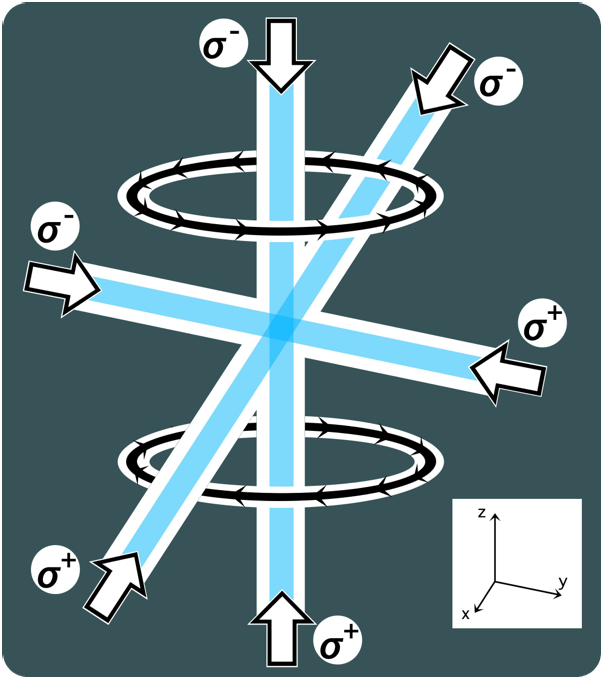
\includegraphics[width=.999\linewidth]{mot.png}
		\caption{Components of a magneto-optical trap, including current-carrying magnetic field coils and counterpropagating circularly polarized laser beams. Diagram taken from~\cite{thesis}}
		\label{fig:mot}
    	\label{fig:themot}
\end{figure}


%%% % % % %%%
\section{The AC-MOT}
\label{sec:acmot}
Citation for Harvey and Murray goes here~\cite{harveymurray}.  Also, myself~\cite{thesis}.
\note{Needs work.}

Here's a diagram of our AC-MOT running one AC-MOT/OP cycle, in Fig.~\ref{fig:acmot}.

\begin{figure}[ht]
	\centering
		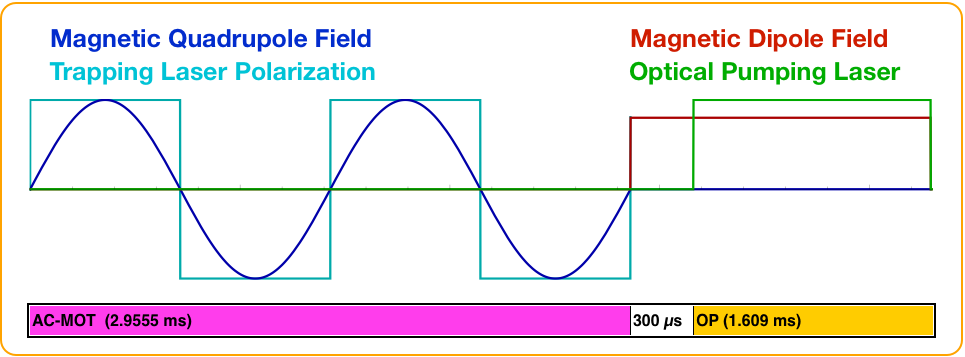
\includegraphics[width=.999\linewidth]{acmot.png}
		\caption{One cycle of trapping with the AC-MOT, followed by optical pumping to spin-polarize the atoms.  After atoms are transferred into the science chamber, this cycle is repeated 100 times before the next transfer.  The magnetic dipole field is created by running parallel (rather than anti-parallel as is needed for the MOT) currents through the two coils.}
		\label{fig:acmot}
\end{figure}


Normal MOTs are DC-MOTs.  They just sort-of go.  It's continuous.  We used an AC-MOT though!  The point of an AC-MOT is to shut off the magnetic field as quickly as possible.  With a well-controlled and uniform magnetic field, we can optically pump the atoms, which I think I'm going to describe in the upcoming section~(\ref{sec:op}).

Sadly, this also removes our trapping mechanism.  We could keep the optical molasses after the field is off if we wanted to, but we don't, because we wouldn't be able to optically pump the atoms then.  But at least the atoms are cold-ish (we can measure!  I think it's done indirectly in that one table, or for realsies in Ben's thesis), so we can let them just chill for a little while before we have to re-trap them.  Don't lose too much.  \aside{How much do we lose?  Have we quantified that somewhere?  Probably.}

Anyway, the idea of the AC-MOT is to run a sinusoidal current through your anti-Helmholtz coils.  You'll get eddy currents in your nearby metal *stuff* when you have a changing current, and those will *also* make a magnetic field. So, the idea with an AC-MOT is that with a sinusoid, you have clear control over what the eddy currents are actually doing, and you can just shut the current off when the eddy currents are zero (current in the anti-Helmholtz coils will be close to zero at this time too, depending on frequency of the sinusoid...), so you can reduce the size of the eddy currents by like an order of magnitude.  Eddy currents in general take a while to die away, so it's good to make them as small as possible.  ...Also, eddy currents making a magnetic field will screw up your optical pumping, because .... um, reasons?  I think it's not just the detuning, it's also something about the Larmor precession.  


\note[color=done]{Removed `Photoionization as a Probe' section from the `Intro to Atomic Physics' section, because John says it's horribly wrong anyhow.  Plus, it's redundant with the `Photoionization Laser' section.}
%\section{Photoionization as a Probe}
%\label{sec:photoprobe}
%\note[color=jb]{JB on 3.5 `Photoionization as a probe' (that's this section!):
%\\
%You describe this well in 4.4 "Photoionization laser"
%\\
%So I recommend strongly you cut  the whole 3.5 section,
%because it's incomplete, and what you
%have contains errors.
%\\ ... \\
%Here are things there are not time to understand:
%\\ ... \\
%about 1/3 of the MOT atoms are excited, not 'a large fraction'
%\\ ... \\
%yes, we've intentionally polarized the OP laser to be circular so the
%atoms will be polarized. We've also picked the S 1/2 to P1/2 so that the
%fully stretched S1/2 $F=2$ $m_F=2$ state is dark. (Unlike the MOT, where we
%need the P3/2 state so that atoms never go dark,  or the force would stop.)
%But we agreed above not to talk about this.
%\\ ... \\
%"We have a photodiode(?) to observe what fraction of things get photoionized overall."
%\\ ... \\
%no, we look at the photoionization rate, for which we have the ion vs. photodiode TOF (`photodiode' looks at when the bursts of light occur)
%}
%
%So, the photoionization laser.  It ionizes only $\approx 1\%$ of the atoms, so it's mostly non-destructive.  
%
%For atoms in a MOT, it can give a projection of the trap position.  At least, it can if you add some MCPs with delay lines, and an electric field.  Also, the atoms have to be excited or they don't get photoionized this way.  That's because at any given time, a large fraction of the trapped atoms are in the excited state, so it works.
%
%For polarized or partially polarized atoms, absorption stops, because of selection rules.  We've intentionally polarized the laser to do this.  I think.  \aside[color=todoblue]{*Have* we even polarized the photoionization laser in any particular way?  I'm not sure we even have.  Why doesn't it absorb?  When it's stretched, it's not just all in the excited state!  It's...stretched.  Do angular momentum selection rules even apply if the electron is going into the continuum?}
%
%\note{Include a picture of the trap.  Possibly on both the rMCP and the eMCP.  Also, maybe a thing for the polarization as a function of time?  But I don't really need to do that, because it's in the paper.}
%
%Anyway, the probing only works if you have a detector to see what things.  We have a photodiode(?) to observe what fraction of things get photoionized overall.  This gives us polarization.  We also have an MCP with delay lines, and an electric field to guide (positive) ions into it.  And another MCP with delay lines on the other side of the electric field, to collect the electrons removed by photoionization.  Also, the (orbital) electrons removed during beta decay.  The photoionization laser is pulsed.  So, when there's a pulse, we can check whether there was a hit detected in the ion detector and/or the electron detector.  It turns out, we can't check both at the same time, because our two detectors hate each other.  They're natural enemies, really.  Turns out, the ion detector is better at measuring the polarization, and the trap position.  Because reasons.  \aside[color=org]{But it's worse for $\Abeta$ and $\bFierz$, because .... reasons that probably shouldn't go in this chapter.}  Anyway, during the 2014 run, we spent like half of the beamtime collecting ions and half collecting electrons.  \aside[color=org]{This also doesn't go in this section.}



